\documentclass[UTF8]{ctexart}
\usepackage{bookmark}
\usepackage{hyperref}
\usepackage{geometry}
\geometry{a4paper,scale=0.8}
\usepackage{ctex}
\usepackage[style=caspervector,backend=biber,utf8]{biblatex}
\addbibresource{reference.bib}
\usepackage{booktabs}
\usepackage{array}
\usepackage{fancyhdr}
\pagestyle{fancy}
\fancyhf{}
\renewcommand\footrulewidth{1pt}
\lhead{王铠泽}
\rhead{PB18020766}
\chead{\href{mailto:volar@mail.ustc.edu.cn}{volar@mail.ustc.edu.cn}}
\rfoot{中国科学技术大学}
\lfoot{\today}
\usepackage{graphicx}
\usepackage{float}
\usepackage{subfigure}


\begin{document}

	\centering\textbf{\LARGE{计算物理A第一次作业}}
	
	
	王铠泽\qquad PB18020766
	
		
	\section{作业题目}
	
	\begin{itemize}
		\item 用$Schrage$方法编写随机数子程序,用连续两个随机数作为点的坐标值绘出若干点的平面分布图。再用$\langle x_k\rangle$测试均匀性。(取不同量级的$N$值,讨论偏差与$N$的关系)、$C(l)$ 测试其2维独立性。(总点数$N>10^7$)。
	\end{itemize}
	
	\section{实现方法}
	
	\begin{itemize}
		\item Lehmer线性同余随机数产生器
		
		$$I_{n+1}=(aI_n+b)\,mod\,m$$
		$$x_n=I_n/m$$
		在本次实验中,主要采用的是16807产生器(最低标准产生器),即 $a=16807,b=0,m=2^{31}-1$
		\item Schrage方法
		
		为了在计算过程中中间数据不溢出,使用$Shrage$方法来求取余数。
		
		$$az\,mod\, m=\left\{
		\begin{array}{lcl}
		a(z\,mod\,q)-r[z/q]       &      &a(z\,mod\,q)-r[z/q] \geq0 \\
		a(z\,mod\,q)-r[z/q]+m&      & otherwise
		\end{array} \right. $$
		
		\item 均匀性检验
		
			\subitem 将产生的$\{\xi\}$序列按如下顺序作为二维平面点集并绘出直观上检验独立性:
		$(\xi_1,\xi_2),(\xi_3,\xi_4),(\xi_5,\xi_6)...$
		
		\item 独立性检验

		\subitem 本次实验中,通过随机变量$x$的各阶矩和关联函数,以及检验统计量$\chi^2$来验证独立性。
		理想情况下,
		$$\langle x^{n} \rangle=\frac{1}{n+1}$$
		$$C(l)=\frac{\langle x_n \rangle \langle x_{n+l} \rangle-\langle x_n \rangle^2}{ \langle x_n^2 \rangle-\langle x_n \rangle^2}=0$$
	\end{itemize}
	\section{程式说明}
	
	\begin{itemize}
		\item Schrage.c 
		
		该程式是使用基于16807产生器生成指定数目($N$)随机数并计算各阶矩和关联系数的程式。
		
		包含以下函数:
		\subitem int shrage (int a, int m, int In)
		
		返回值是 $aI_n\,mod\,m$
		
		\subitem int initial (int n)
		
		$n=0$ 为默认种子 $I_0=1$, $n=1$ 为时间种子生成 $I_0$
		
		\subitem int main()
		
		main函数分为三个模块,分别是生成随机数,计算各阶矩(1-4阶)和关联函数[C(0)-C(20)]。	
		
		\item Correlation.c 
		
		这是后续用于生成大量的关联系数的程式。由此生成$10^4,10^5$个$C(l)$探究规律。
		
		\item time\_seed.txt
		
		该文本文件显示的是最后一次调用时间种子时对应的原始数据。
		
		\item data.txt
		
		这类文本文件包括了不同 $N$ 下产生的随机数和各类相关物理量的详细数据。
		
		
	\end{itemize}
	
	\section{计算结果}
	在调用时间种子情况下,得到如下结果。
%	\begin{figure}[H]
%	\centering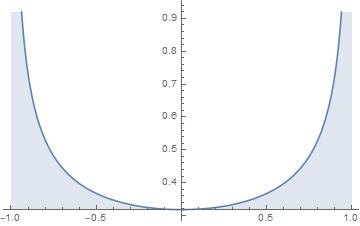
\includegraphics[width=2in]{1.jpg}
%	\caption{something}\label{fig:1}
%	\end{figure}
	\subsection{散点分布情况}
	\begin{figure}[H]
		\centering  %图片全局居中
		\subfigure[$N$=100]{
			\label{N=100}
			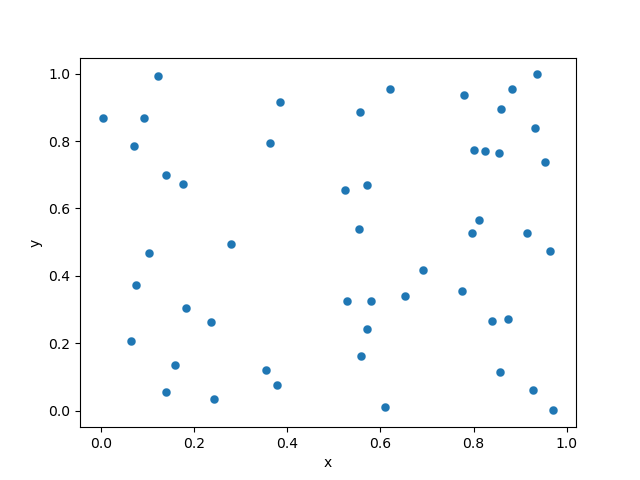
\includegraphics[width=0.45\textwidth]{../N=100.png}}
		\subfigure[$N$=1000]{
			\label{N=1000}
			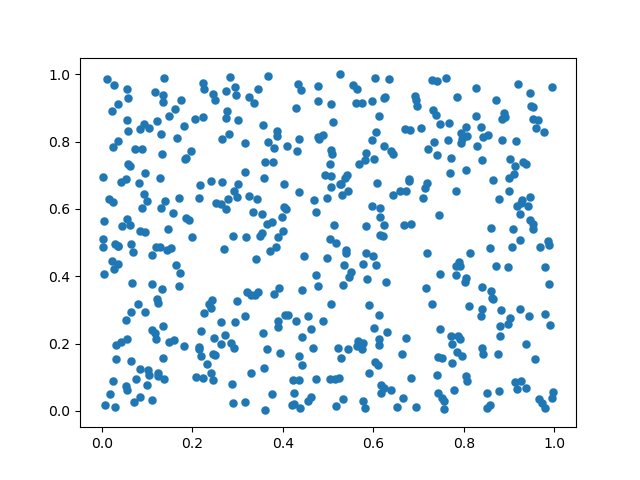
\includegraphics[width=0.45\textwidth]{../N=1000.png}}
		\subfigure[$N$=10000]{
			\label{N=10000}
			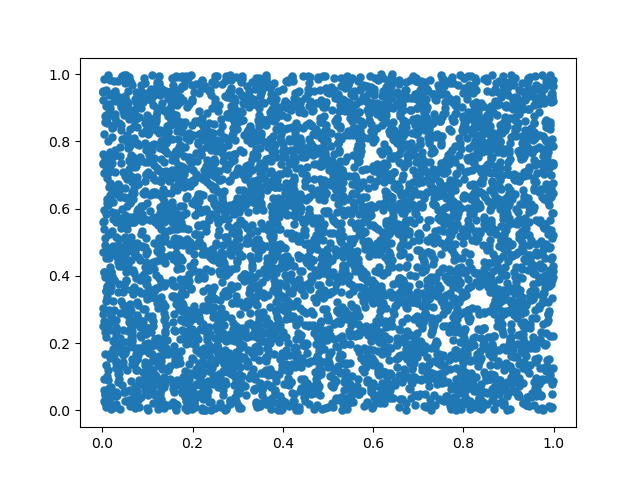
\includegraphics[width=0.45\textwidth]{../N=10000.png}}
		\subfigure[$N$=10000000]{
			\label{N=10000000}
			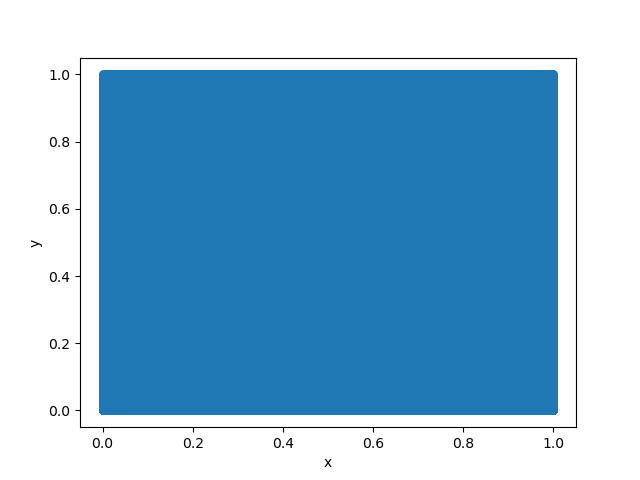
\includegraphics[width=0.45\textwidth]{../N=10000000.png}}
		\caption{不同$N$下的散点分布情况}
		\label{N}
	\end{figure}
	
	
	当点数达到10000量级以后,可以认为是均匀铺满二维平面,说明16807产生器生成随机数比较理想。
	
	\subsection{不同抽样点数 $N$ 下各阶矩和理想情况的比较}
	
	\begin{table}[H]
		\centering
		\setlength{\tabcolsep}{10mm}{
		\begin{tabular}{@{}llll@{}}
			\toprule
			$k$&$x^k$& $x^k-\frac{1}{k+1}$&$\frac{1}{\sqrt{N}}$ \\ \midrule
			1&0.511107 & 0.011107&0.100000\\
			2&0.352723	& 0.019389&0.100000\\
			3&0.268752	&0.018752&0.100000\\
			4&0.215926	&0.015926&0.100000 \\ \bottomrule
			
		\end{tabular}}
		\caption{$N$=100的$\langle x^k \rangle$平均值和误差}
	\end{table}

	\begin{table}[H]
		\centering
		\setlength{\tabcolsep}{10mm}{
			\begin{tabular}{@{}llll@{}}
				\toprule
				$k$&$x^k$& $x^k-\frac{1}{k+1}$&$\frac{1}{\sqrt{N}}$ \\ \midrule
				1	&0.496715	&-0.003285& 0.010000\\
				2	&0.331324	&-0.002009& 0.010000\\
				3	&0.248791	&-0.001209& 0.010000\\
				4	&0.199217	&-0.000783& 0.010000\\ \bottomrule
		\end{tabular}}
		\caption{$N$=1000的$\langle x^k \rangle$和误差}
	\end{table}

	\begin{table}[H]
	\centering
	\setlength{\tabcolsep}{10mm}{
		\begin{tabular}{@{}llll@{}}
			\toprule
			$k$&$x^k$& $x^k-\frac{1}{k+1}$&$\frac{1}{\sqrt{N}}$ \\ \midrule
			1	&0.499714	&-0.000286& 0.010000\\
			2	&0.334310	&0.000976& 0.010000\\
			3	&0.251595	&0.001595& 0.010000\\
			4	&0.201846	&0.001846& 0.010000\\ \bottomrule
	\end{tabular}}
	\caption{$N$=10000的$\langle x^k \rangle$和误差}
\end{table}

	\begin{table}[H]
		\centering
		\setlength{\tabcolsep}{10mm}{
			\begin{tabular}{@{}llll@{}}
				\toprule
				$k$&$x^k$& $x^k-\frac{1}{k+1}$&$\frac{1}{\sqrt{N}}$ \\ \midrule
			1	&0.499963	&-0.000037&0.0003162\\
			2	&0.333304	&-0.000029&0.0003162\\
			3	&0.249988	&-0.000012&0.0003162\\
			4	&0.200005	&0.000005&0.0003162\\
			 \bottomrule
		\end{tabular}}
		\caption{$N$=10000000的$\langle x^k \rangle$和误差}
	\end{table}
  通过上述分析可得到产生随机数的矩和理想值之误差满足$\delta x=O(\frac{1}{\sqrt{N}})$,甚至还略小一两个数量级。

	\subsection{用 $C(l)$ 测试其独立性}
		$\frac{1}{\sqrt{N}}$=0.0003162
		\begin{table}[H]
		\centering
		\setlength{\tabcolsep}{10mm}{
			\begin{tabular}{@{}llll@{}}
				\toprule
				$k$&$C(k)$&$k$&$C(k)$\\ \midrule
				0 &	1.000000 &
			1 &	0.000280\\
			2 &	0.000218 &
			3 &	-0.000389\\
			4 &	-0.000154 &
			5 &	-0.000148\\
			6 &	-0.000488 &
			7 &	-0.000273\\
			8 &	-0.000010 &
			9 &	0.000426\\
			10 &	0.000516 &
			11	 &-0.000012\\
			12	 &-0.000010 &
			13 &	0.000028\\
			14	 &-0.000522 &
			15	 &0.001037\\
			16 &0.000134 &
			17 &	0.000220\\
			18	 &0.000200 &
			19 &	0.000340\\
			20	 &0.000354 &
			& \\
			
				\bottomrule
		\end{tabular}}
		\caption{$N=10000000$时关联函数$C(k)$的取值}
	\end{table}
	$N$比较大($N$$\geq$$10^7$)的情况下,关联很弱,基本上都在$O(\frac{1}{\sqrt N})$量级。
	
\begin{flushleft}
		为了探究$C(l)$的分布,分别生成了$N=10^4$和$N=10^5$个关联系数$C(1)\sim C(N)$。
	下面给出一些计算结果。
	\subsubsection{$C(l)-l$关系}
\end{flushleft}
	
		\begin{figure}[H]
			\centering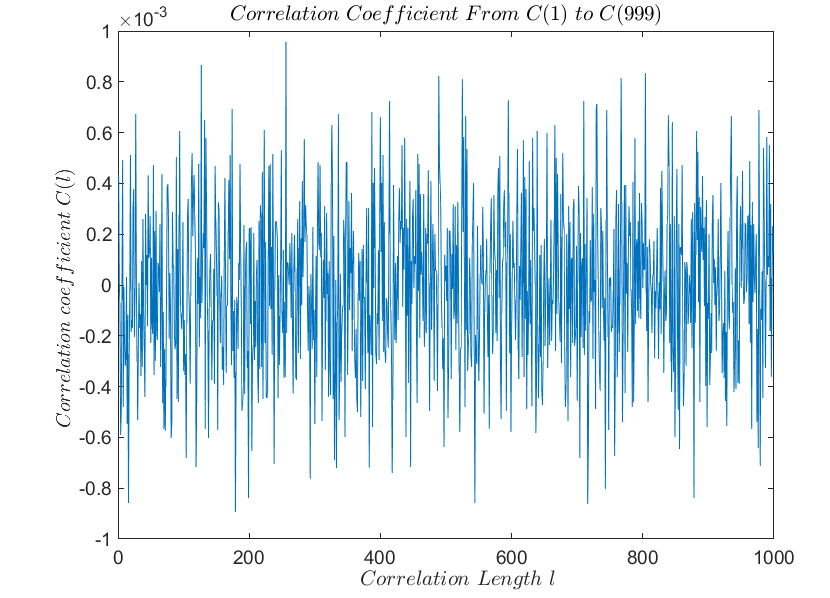
\includegraphics[width=4in]{../figure/cor.png}
			\caption{$C(l)-l$函数图线}
		\end{figure}
	分布较为杂乱,考虑做出其频谱图:
		\begin{figure}[H]
			\centering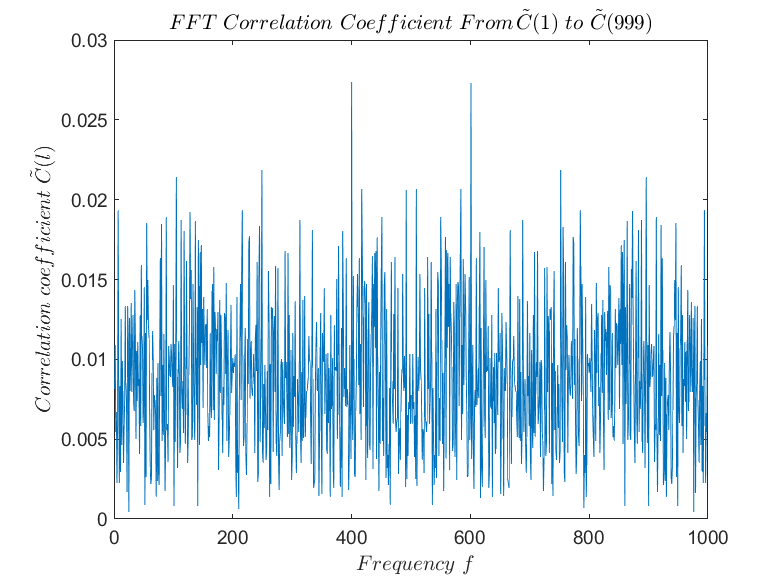
\includegraphics[width=4in]{../figure/fft.png}
			\caption{频域$\tilde{C}(l)-l$函数图线}
		\end{figure}
	\begin{flushleft}
		频域上虽然也是一个剧烈震荡的分布,但是可以看出是左右对称并且可能有周期分布。目前暂时没有看出其他关于$C(l)-l$关系的特别的性质。
	\end{flushleft}
	
	\subsubsection{误差分布}
	\begin{flushleft}
		如果将各个$C(l)$地位等同起来,只看误差的直方图分布,我们可以得到更清晰有趣的结论。看起来误差的分布像是一个正态分布。
	\end{flushleft}
	
	\begin{figure}[H]
		\centering  %图片全局居中
		\subfigure[$\mbox{关联系数总个数}=10^4$]{
			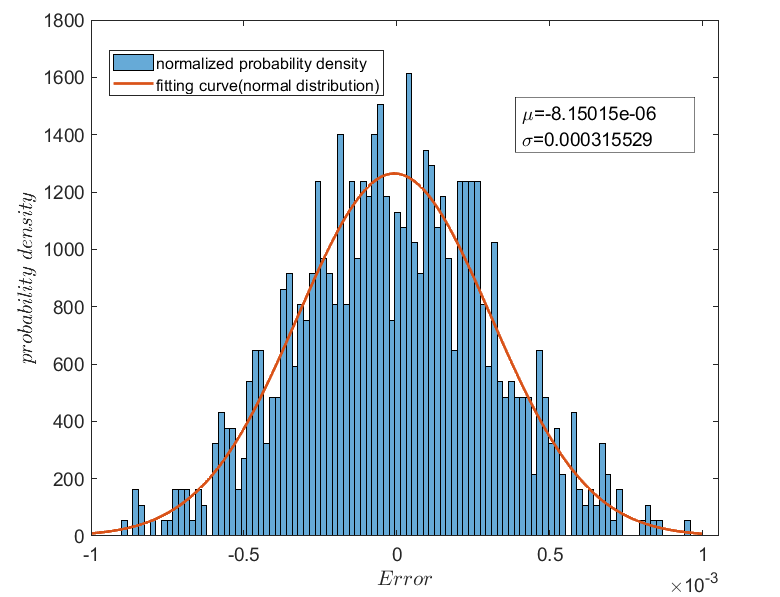
\includegraphics[width=0.6\textwidth]{../figure/normal.png}}
		\subfigure[$\mbox{关联系数总个数}=10^5$]{
			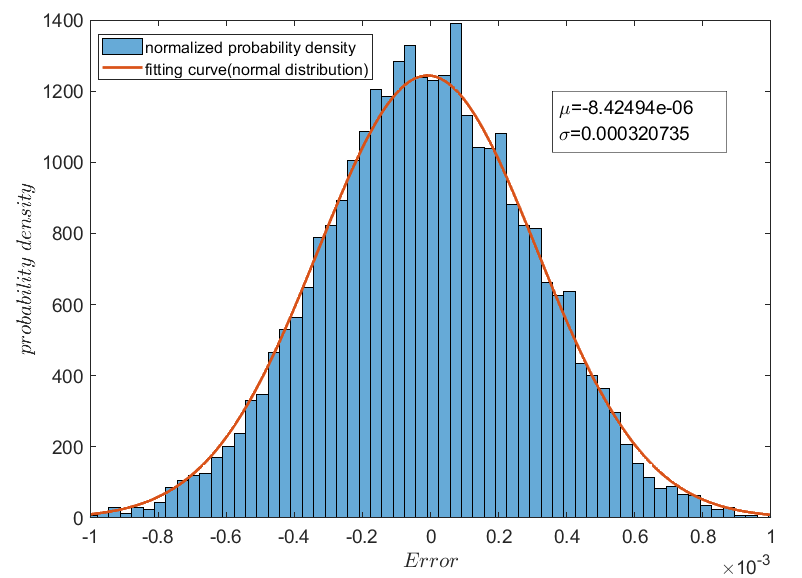
\includegraphics[width=0.6\textwidth]{../figure/normal2.png}}
		\caption{误差分布}

	\end{figure}
	
\begin{flushleft}
		这个正态分布的参数值$\mu\approx0,\sigma\approx0.00032$。这符合我们对多个随机序列检验的认知。具体的数学证明还有待推导。
\end{flushleft}
	
	\subsection{$\chi^2$检验}
	
	\begin{flushleft}
		对于默认种子$I_0=1$,生成 $10^7$ 个随机数。将二维平面上[0,1]$\times$[0,1]区域分成 5 $\times$ 5=25个小正方形,进行自由度为24的$\chi^2$检验。得到的$\chi^2= 16.732340$。查阅资料得知:
	\end{flushleft}
	$$\chi_{24}(0.995)=9.886,\chi_{24}(0.99)=10.856,\chi_{24}(0.975)=12.401,\chi_{24}(0.95)=12.848,\chi_{24}(0.90)=15.659$$
	
	\begin{flushleft}
		选用不同时间种子统计出的$\chi^2$也并不相同,有时能达到13.9000这样的数值。
		比较可得知,虽然在其他检验中16807产生器还是算比较良好,但是在$\chi^2$检验下,其只有大约90\%的置信概率。
	\end{flushleft}
	\section{其他}
\begin{flushleft}
	
	选择好的线性同余器参数尤为重要,一组好的参数能大大提高重复周期。一般而言,不恰当的 $a$,$b$ 取值会导致二维分布是在几条分立线上,而非几乎铺满整个平面。下面给出的是$a=7,b=2$的结果。
\end{flushleft}
	
	\begin{figure}[H]
			\centering
			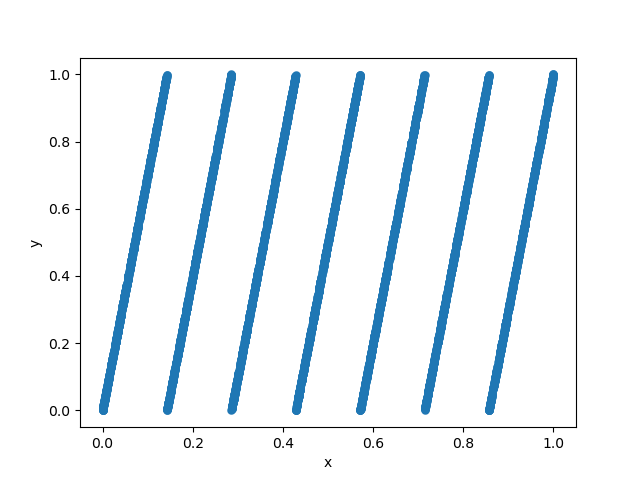
\includegraphics[width=4in]{../N_=10000.png}
			\caption{$a=7,b=2,N=10000$}\label{ap}
	\end{figure}

	但是值得一提的是,这组随机数的各阶矩和关联系数都体现出较为良好的特征。
	
	\begin{table}[H]
		\centering
		\setlength{\tabcolsep}{10mm}{
			\begin{tabular}{@{}llll@{}}
			\toprule
			$k$&$x^k$& $\frac{1}{k+1}-x^k$&$\frac{1}{\sqrt{N}}$ \\ \midrule
			1&0.498572 & 0.001428&0.010000\\
			2&0.331881	& 0.001452&0.010000\\
			3&0.248678	&0.001322&0.010000\\
			4&0.198830	&0.001170&0.010000 \\ \bottomrule
		\end{tabular}
	
	\caption{$a=7,b=2,N=10000$时的矩}}
	\end{table}

	\begin{table}[H]
		\centering
		\setlength{\tabcolsep}{10mm}{
			\begin{tabular}{@{}llll@{}}
				\toprule
				$k$&$C(k)$&$k$&$C(k)$\\ \midrule
				0  &  1.000000&
				1  &  0.160635\\
				2   & 0.034297&
				3  &0.014033\\
				4  &0.001413&
				5   &0.009139\\
				6   &0.008559&
				7   &-0.007316\\
				8   &-0.000741&
				9   & -0.016261\\
				10  & -0.004097&
				11  & -0.013075\\
				12  & -0.000324&
				13  & -0.007607\\
				14  & -0.013594&
				15  & -0.016038\\
				16  & 0.017166&
				17  & -0.002381\\
				18  & -0.005216&
				19  & -0.022513\\
				20  & -0.003828&
				&  \\
			
				\bottomrule
		\end{tabular}}
		\caption{$N=10000$时关联函数$C(k)$的取值}
	\end{table}

\begin{flushleft}
\textbf{	$C(l)$表示的关联比较弱。}
\end{flushleft}
	\begin{flushleft}
		\textbf{在进行$\chi^2$检验时,$\chi^2=735.540000$,明显这不是一组独立随机数。}
	\end{flushleft}

	\section{总结}
	\begin{itemize}
		\item 16807产生器生成的随机数序列随即独立性比较良好,在置信概率大约90\%下可以认为其是独立的
		
		\item 良好随机数关联函数的误差分布可能是一个正态分布。
		
		\item 单独一种独立性检验不能非常完美地刻画一组随机数的性质良好与否,上面所举的就是一个很好的反例。考量一组随机数的质量应当从多个方面考虑/
	\end{itemize}
	\clearpage
\end{document}